\documentclass[a4paper, 12pt]{article}

\usepackage{geometry}
\usepackage{amsmath}
\usepackage{gvv}

\graphicspath{{figs/}}
\title{Question 2.7.12}
\author{AI25BTECH11040 - Vivaan Parashar}
\date{\today}

\begin{document}

\maketitle

\section{Question: }
Find the area of the triangle formed by joining the midpoints of the sides of the triangle ABC, whose vertices are A$(0, -1)$, B$(2, 1)$, and C$(0, 3)$

\section{Solution: }
Let us start by finding the midpoints, let's call them D, E and F.
The midpoint formula is: (Here the vectors represent position vectors of the points from the origin)
\begin{align}
    \vec{D} = \frac{\vec{A}+\vec{B}}{2} \\
    \vec{E} = \frac{\vec{B}+\vec{C}}{2} \\
    \vec{F} = \frac{\vec{C}+\vec{A}}{2} \\
    \therefore \vec{D} = \myvec{1       \\ 0}, \vec{E} = \myvec{1 \\ 2}, \vec{F} = \myvec{0 \\ 1}
\end{align}
Now the area formula for a triangle with vertices at $\vec{P}$, $\vec{Q}$ and $\vec{R}$ is given by:
\begin{align}
    \text{Area} = \frac{1}{2} \norm{(\vec{P} - \vec{Q}) \times (\vec{P} - \vec{R}) }                                                                                        \\
    \therefore \text{Area of } \triangle DEF = \frac{1}{2} \norm{(\vec{D} - \vec{E}) \times (\vec{D} - \vec{F}) }                                                           \\
    = \frac{1}{2} \norm{\left( \frac{\vec{A}+\vec{B}}{2} - \frac{\vec{B}+\vec{C}}{2} \right) \times \left( \frac{\vec{A} + \vec{B}}{2} - \frac{\vec{C}+\vec{A}}{2}\right) } \\
    = \frac{1}{2} \norm{\left( \myvec{1                                                                                                                                     \\ 0} - \myvec{1 \\ 2} \right) \times \left( \myvec{1 \\ 0} - \myvec{0 \\ 1} \right) }\\
    = \frac{1}{2} \norm{\myvec{0                                                                                                                                            \\ -2} \times \myvec{1 \\ -1} }\\
    = \frac{1}{2} |0 - 2| = 1
\end{align}

\section{Diagram: }
The diagram showing the triangle ABC and the triangle DEF is shown below:
\begin{figure}[h]
    \centering
    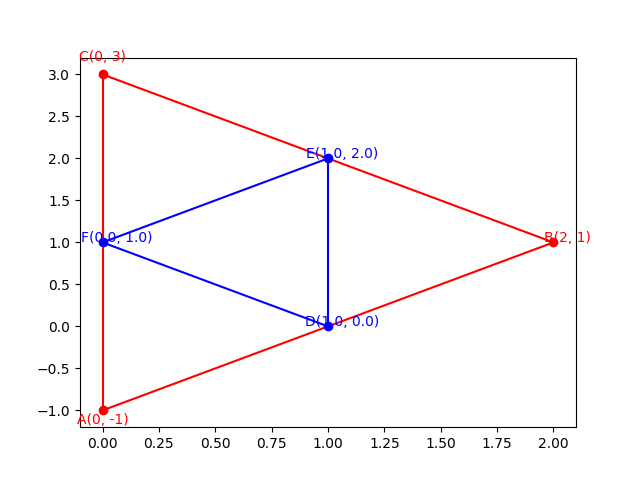
\includegraphics[width=0.8\linewidth]{figs/triangle_diagram.png}
    \caption{Diagram showing the triangle ABC and the triangle DEF.}
    \label{fig:triangle_diagram}
\end{figure}

\end{document}
